\section{Versuchsdurchführung und Auswertung}
	\subsection{Einstellen der Betriebsparameter}
		Um die folgenden Messungen unter möglichst günstigen Bedingungen durchführen zu können, wurden zunächst unter Anweisung des Betreuers die Betriebsparameter der Ionenfalle überprüfung und gegebenenfalls optimiert:
		\begin{itemize}
			\item linke Potentialwand $U_0 = \unit[11,857]{kV}$
			\item Potentialtopf ($\hat{=}$ Beschleunigungsspannung) $U_A = \unit[11,707]{kV}=U_B$
			\item rechte Potentialwand $U_{B1} = \unit[12,007]{kV}$
			\item Extraktionszeit $t_{ext} = \unit[20]{ms}$
		\end{itemize}
		Da die Abhängigkeit der Argonionisationen von Arbeitsdruck und Ionisationszeit innerhalb des Strahlrohrs untersucht werden soll, werden diese in den folgenden Abschnitten genauer spezifiziert. Abbildung \ref{fig:potentialkasten} skizziert nochmals die Potentialverhältnisse entlang der Strahlachse.
		\begin{figure}
			\centering
			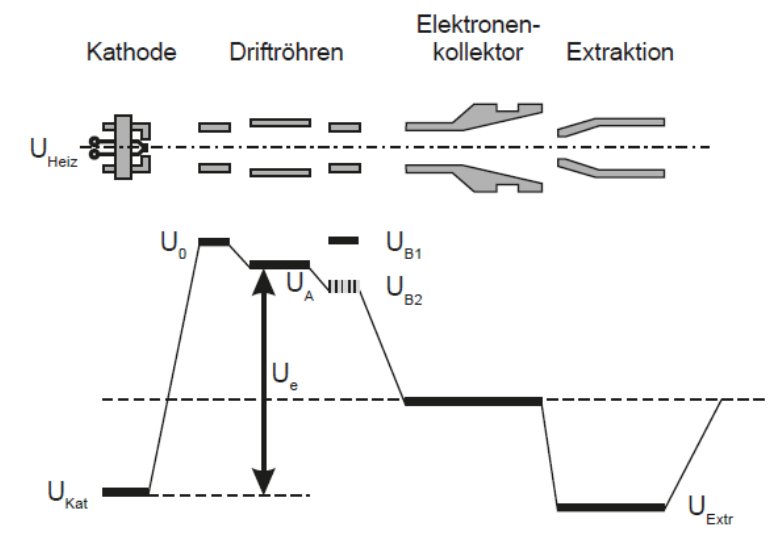
\includegraphics[width=0.8\linewidth]{pic/potentialkasten}
			\caption{Elektrodenanordnung (oben) mit zugehörigem Potentialverlauf in der Ionenfalle.\cite{PA}}
			\label{fig:potentialkasten}
		\end{figure}
		
	\subsection{Aufnahme und Analyse eines Übersichtsspektrums}
		Um die einzelnen Ionisationszustände des Argons sauber voneinander trennen zu können, ist es notwendig zu wissen, wie man den Strom des 90°-Dipol-Magneten wählen muss. Im Experiment sollen die Ionen Ar$^{8+}$ bis Ar$^{18+}$ untersucht werden. Mit Hilfe von Formel (\ref{eq:radius}) wird das Magnetfeld abgeschätzt, um die gewünschten Ionen auszufiltern. Es ergibt sich ein Messintervall von $B = 50,4 \dots \unit[75,6]{mT}$, wobei die untere Grenze den höchsten Ionisationszustand Ar$^{18+}$ und die untere Grenze den niedrigsten Zustand Ar$^{8+}$ herausfiltert. Die Einstellung dieser Magnetflussdichten erfolgt über die Variation des Spulenstroms von $\unit[17,3]{A}$ bis $\unit[27,2]{A}$. 
		Bei der ersten Messung wurde die Ionisationszeit mit $t_{ion} = \unit[380]{ms}$ zu hoch gewählt, um damit niedrigere Ladungszustände als Ar$^13$ zu erzeugen. Dies hat sich allerdings erst im zweiten Versuchsteil herausgestellt. Der Vollständigkeit halber zeigt Abbildung \ref{fig:7e-9} das dabei entstandene Übersichtsspektrum bei einem Arbeitsdruck von $p = \unit[7\cdot 10^{-9}]{mbar}$. Die Ladung $Q$ wurde dabei über 5 Zyklen integriert.\\
		\begin{figure}
					\centering
					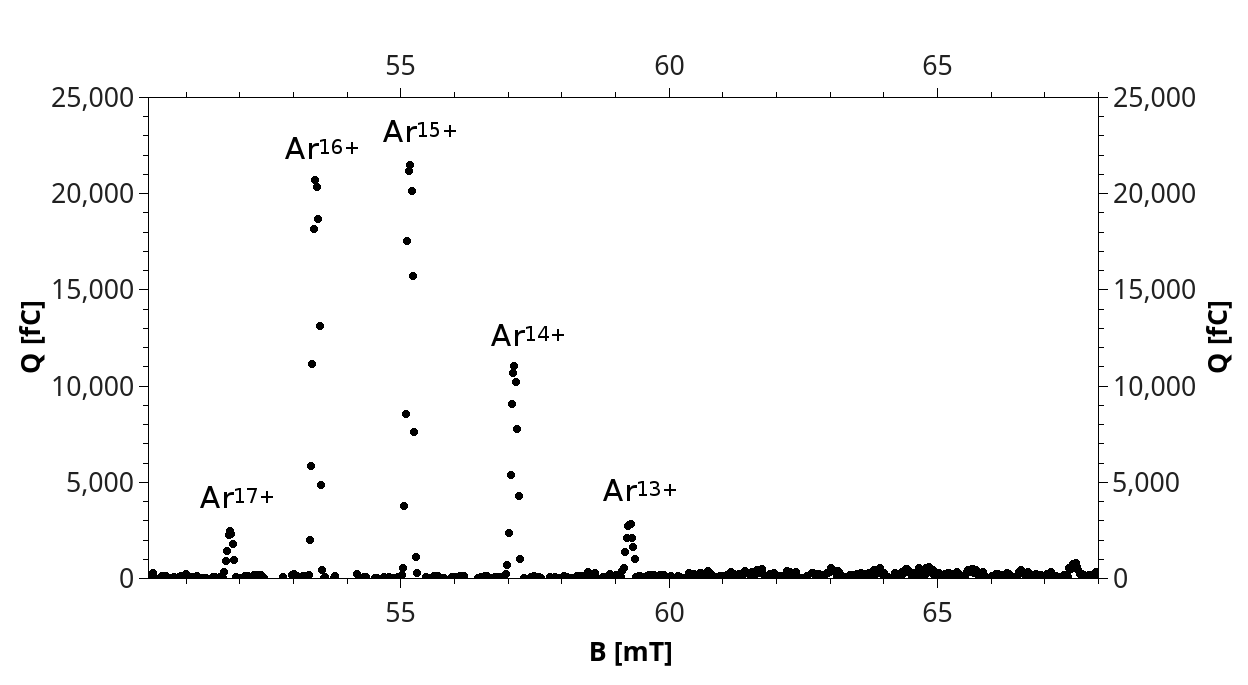
\includegraphics[width=\linewidth]{pic/7e-9_beschriftet}
					\caption{Übersichtsspektrum bei $p = \unit[7\cdot 10^{-9}]{mbar}$ und $t_{ion} = \unit[380]{ms}$. Die Peaks niedriger Ladungszustände verschwinden aufgrund der zu hohen Ionisationszeit.}
					\label{fig:7e-9}
		\end{figure}
		Die Messung wurde mit einer niedrigeren Ionisationszeit $t_{ion} = \unit[80]{ms}$ und einem erhöhten Arbeitsdruck $p = \unit[2\cdot 10^{-8}]{mbar}$ wiederholt. Diese Wahl maximiert die Häufigkeit von mittleren Ionisationszuständen um Ar$^{12}$ und ermöglicht die Messung aller möglicher Peaks. Zugleich soll diese Einstellung den Einfluss des Drucks untersuchen. Abbildung \ref{fig:2e-8} zeigt das zugehörige Übersichtsspektrum, bei dem ebenfalls über 5 Zyklen integriert wurde.
		\begin{figure}
							\centering
							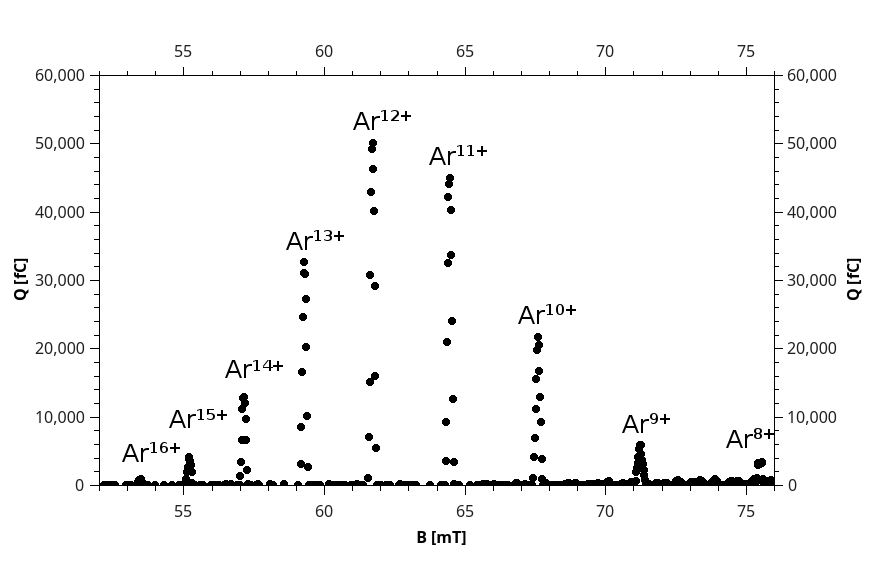
\includegraphics[width=\linewidth]{pic/2e-8_beschriftet}
							\caption{Übersichtsspektrum bei mittlerem Arbeitsdruck $p = \unit[2\cdot 10^{-8}]{mbar}$ und $t_{ion} = \unit[80]{ms}$. Alle gewünschten Peaks sind erkennbar, da nun mittlere Ladungszustände am häufigsten auftreten.}
							\label{fig:2e-8}
		\end{figure}
		